\chapter{¿Qué es una simulación? Gazebo y SITL}
\label{cap:simulacion}

\begin{enpocas}
Por qué se simula, qué hace Gazebo, cómo se describe un robot, qué son los plugins, el tiempo simulado
y qué significa que PX4 corra ``en el lazo'' (SITL).
\end{enpocas}

\section{¿Por qué simular?}

Una búsqueda real necesita un dron, un bosque, voluntarios que hagan de personas perdidas y permisos; y
un error de programación puede estrellar el dron. En simulación:
\begin{itemize}
  \item los choques no cuestan nada;
  \item se repite exactamente el mismo bosque, con las mismas personas y el mismo viento, para comparar
        dos estrategias en igualdad de condiciones (imposible al aire libre);
  \item se conoce la verdad: dónde está cada persona, para medir el error de localización;
  \item se pueden correr cientos de vuelos sin supervisión (capítulo~\ref{cap:experimental}).
\end{itemize}

\begin{recuerda}
La simulación no reemplaza el vuelo real: lo prepara y permite responder preguntas que en campo
costarían meses.
\end{recuerda}

\section{Gazebo}

\textbf{Gazebo Harmonic} calcula en cada paso la física (motor DART), dibuja la escena (OGRE~2), genera
las lecturas de los sensores (cámara, IMU, GPS, LiDAR) y ejecuta \emph{plugins}: los motores, el
viento (\cod{WindEffects}), el piloto de ArduPilot o el selector de motores del proyecto.

\begin{figure}[H]
\centering
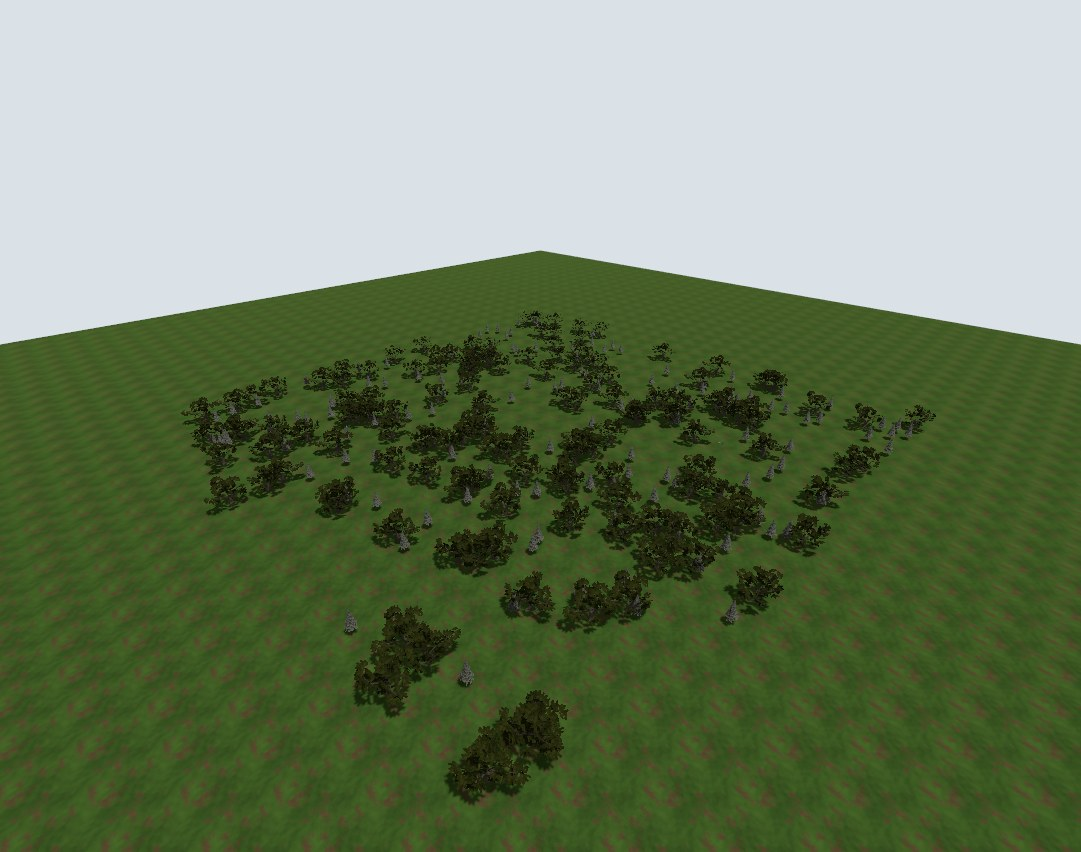
\includegraphics[width=0.75\textwidth]{gz_bosque_aereo.jpg}
\caption{El bosque de la simulación (oclusión media) visto desde lejos.}
\end{figure}

\section{SDF: cómo se describe un robot}

Robots y mundos se escriben en \textbf{SDF} (XML): eslabones con masa, inercia, forma visual y forma de
colisión; articulaciones; sensores; plugins. El x500 del proyecto es el de PX4 con tres cambios
(capítulo~\ref{cap:x500}): la cámara bajo los patines, viento habilitado y un LiDAR.

\section{Personas con etiqueta}

Gazebo puede asignar una \textbf{etiqueta} a cada modelo (sistema \cod{Label}). Las personas llevan la
etiqueta~1. Una cámara especial de Gazebo (\emph{boundingbox camera}) devuelve entonces el recuadro de
la parte \emph{visible} de cada persona: así se etiquetaron solas las 3000 imágenes del dataset del
detector (capítulo~\ref{cap:detector}).

\section{Tiempo simulado}

La simulación tiene su propio reloj: si la computadora es lenta, todo va más despacio pero los resultados
no cambian. El \textbf{factor de tiempo real} mide la proporción. Todos los nodos usan el reloj de
Gazebo (\cod{use_sim_time}).

\section{SITL: el piloto real en la computadora}

En \textbf{SITL} (\emph{software in the loop}) el mismo programa del piloto automático que volaría en
el dron real ---PX4 o ArduCopter--- corre en la computadora y recibe los sensores simulados. Lo que se
prueba aquí es casi lo que volará. El paso siguiente sería HITL: el controlador de vuelo físico
conectado a la simulación.

\begin{leccion}
PX4 trae su propia configuración de Gazebo, que carga un sistema de video (\cod{GstCameraSystem}). Si
el codificador se atora, acumula cuadros de la cámara: llegó a 110~MB/s, 23~GB en minutos, y el sistema
operativo terminó matando la simulación (y otra que estaba abierta). Ahora el \emph{launch} abre Gazebo
sin esa configuración y conecta PX4 a ese Gazebo (\cod{PX4_GZ_STANDALONE}).
\end{leccion}
